\documentclass[conference]{IEEEtran}
\IEEEoverridecommandlockouts
\usepackage{cite}
\usepackage{times}
\usepackage{url}
\usepackage{graphicx}
\usepackage{amsmath}
\usepackage{booktabs}
\usepackage{array}

\begin{document}
\title{Physics-Prior Latent World Models for Reliable Long-Horizon UAV Prediction under Out-of-Distribution Wind: Mid-Term Progress Report}

\author{
\IEEEauthorblockN{Chethan}
\IEEEauthorblockA{Department of Computational and Data Sciences\\
Indian Institute of Science, Bangalore, India\\
chethan1@iisc.ac.in}
}
\maketitle

\begin{abstract}
Learned world models predict by feeding their own outputs back, so small one-step errors compound over long horizons, and the problem worsens when conditions differ from training. This thesis asks whether the known rigid-body dynamics of a quadrotor, used as a prior inside a latent world model, make long-horizon prediction under out-of-distribution (OOD) wind more reliable. The model is $\dot s = f_{\mathrm{phys}}(s,u) + d_\theta(h,s,u)$. The work so far has concentrated on building trustworthy evidence: a physically validated, reproducible data generator in Isaac Sim, a quality-checked pilot dataset, and seven baseline models evaluated per OOD role. On pilot data (63 training episodes) the physics prior helps in distribution (20-step position RMSE 0.036~m against 0.105~m for a pure neural latent model and 0.053~m for physics alone). It does \emph{not} yet help on the primary OOD axis, wind magnitude, where the proposed model (0.166~m) is at the level of physics alone (0.185~m) and worse than a constant-velocity reference (0.050~m). Diagnostics point to the wind range seen in training and to a latent that carries no readable wind information. A larger, wind-diverse dataset of 4,530 episodes is being generated to address this. This report states the results, their limits, the problems met, and the remaining work.
\end{abstract}

\begin{IEEEkeywords}
UAV, quadrotor, world model, physics prior, residual learning, distribution shift, wind
\end{IEEEkeywords}

\section{Introduction}
A quadrotor follows well-known rigid-body dynamics, but aerodynamic drag, wind, actuator lag and parameter error are hard to describe analytically. A latent world model can imagine futures without further interaction, but recursive prediction accumulates error, and the error grows when the wind differs from the training distribution. A physics prior is a natural remedy: gravity, thrust and kinematics stay valid when the wind changes, so the network only has to learn the remainder.

\textbf{Research gap.} Physics-informed learning, residual dynamics for quadrotors and latent world models have each been studied. A controlled comparison of a \emph{pure learned latent} model against a \emph{physics-prior latent} model, under recursive prediction and controlled OOD wind, is comparatively rare. The thesis contributes that comparison, an OOD wind benchmark, and a reliable-imagination-horizon analysis, not a new component.

\textbf{Research questions.} RQ1: does the physics prior improve long-horizon reliability under OOD wind? RQ2: under which OOD conditions is the benefit largest? RQ3: how sensitive is the benefit to nominal-model accuracy and data amount? RQ4 (extension): can predictive uncertainty flag the unreliable horizon? The primary hypothesis H1 is that the physics-prior model's error grows more slowly; H2 states that the benefit shrinks as the nominal model becomes inaccurate. A negative or conditional result is acceptable if the conditions of failure are identified.

\section{Related Work}
Physics-informed networks for quadrotor dynamics~\cite{gu2024physics} put physical knowledge in the loss rather than in the transition used for imagination. Hybrid models add a learned residual to a first-principles model, as in NeuroBEM~\cite{bauersfeld2021neurobem} (Neural-Fly and Neural Lander follow the same idea), and APHYNITY gives an identifiability argument for minimal-norm residuals. Dreamer-style latent models~\cite{hafner2023mastering} imagine in a fully learned latent state; here the latent is memory attached to an explicit physical state. The data-generation setup follows AirDreamer (OmniDrones, Hummingbird, 200~Hz physics, 20~Hz policy, domain randomisation). The full literature review is in the thesis proposal.

\section{Methodology and Work Done}
\subsection{Model}
The state is $s=(p,v,q,\omega_B)$ (world ENU, body FLU, Hamilton quaternion, body-frame rate). The physics term gives gravity and thrust acceleration and rigid-body rotation, integrated with RK4. The residual acts only on $\dot v$ and $\dot\omega$, since the kinematics are exact; the recurrent latent $h$ is built from a synthetic IMU computed from the model's own state, and the decoder only initialises the state. Training uses a context window with real data followed by a free-running rollout, with a horizon curriculum and a geodesic attitude loss.

\subsection{Baselines}
\begin{table}[h]
\centering\small
\caption{Models compared.}
\begin{tabular}{ll}
\toprule
B0 & hold last state\\
B1 & physics only\\
B2 & pure neural latent dynamics\\
B3 & physics + residual + latent memory (proposed)\\
B4 & physics + residual, no memory\\
B5a/b & learned field / exact kinematics + learned dynamics\\
B6a/b & oracle wrench (no learning / with learning)\\
\bottomrule
\end{tabular}
\end{table}
The central comparison is B2 against B3, with matched data and capacity.

\subsection{Why the data generator became the main work}
An audit (Run~1) found that the first pipeline had never produced a usable dataset (18 episodes of length one) and that wind and drag were silent no-ops. Other defects: angular velocity labelled body-frame while world-frame, mass randomisation not reaching the physics engine, a controller ignoring yaw, windowing at 200~Hz, and training wind of 2--16~m/s instead of the planned 0--4~m/s. The project was therefore restructured into six runs: audit, plan, configuration architecture, validated physics, pilot dataset, and scale-up.

\subsection{Data pipeline}
Every random choice is made at planning time from a seed tree, so an episode is a pure function of one manifest row. The simulator is Isaac Sim 4.1 with OmniDrones and the Hummingbird quadrotor (physics 5~ms, model step 20~ms in the pilot). Project aerodynamics (rotor drag linear in rotor speed, body drag with per-axis $C_D=(1.1,1.1,1.3)$ and projected areas, ground effect) enter through one wrench injector. Wind comes from steady, gust, OU, step, sinusoidal and Dryden components, with realised-statistics guarantees. Counterfactual siblings replay the same action under different wind (Mode~B) or re-run the controller (Mode~A), which separates wind effects from controller reactions. Every force model has an applicability envelope; the rotor-drag envelope is $\mu\le 0.20$ with reduced fidelity between 0.15 and 0.20, and episodes outside an envelope are excluded.

\subsection{Physics validation}
All checks ran inside Isaac Sim (17 Isaac and 250 CPU tests pass). Hover gives 9.810~m/s$^2$ and free fall 0; a 1~N force gives 1.3957~m/s$^2$ against 1.3966 expected; a 3~m/s wind at hover attitude gives 0.9614 against 0.9618; motor-step error is $6\times10^{-8}$; torque responses are within about 0.5\%; repeated episodes are bitwise identical within a process.

\subsection{Pilot dataset and quality}
Pilot v0.5.0 holds 147 episodes (141 completed, 6 ended on ground contact, kept and flagged) with 63 training episodes. The validator reports 0 hard and 0 soft findings; the statistical check shows no NaN, no out-of-limit sample, realised wind within each regime's limits, and a ground-truth Newton-law residual of 0.030~m/s$^2$ (p99). Findings: the Isaac IMU accelerometer carried an extra $-\omega\times v$ term (p99 1.65~m/s$^2$, corrected at generation in v0.6.0); open-loop action--wind correlation was 0.39 (permutation $p=0.085$); domain factors correlated ($|\rho|=0.59$); and OOD roles had only 2--7 independent groups.

\section{Experiments and Results}
\subsection{Setup}
Metric: position RMSE after 20 model steps (0.4~s) from the true initial state, per split role. Limits that apply to everything below: pilot-size data (63 training episodes), 4--7 episodes per OOD role, three seeds for B3, B4 and B5b and one for the others, one dataset for variant comparisons.

\subsection{Results}
\begin{table}[h]
\centering\small
\caption{20-step position RMSE [m], pilot v0.6.0 (mean over seeds for B3).}
\begin{tabular}{lccccc}
\toprule
Model & ID & Mag. & Dir. & Temp. & Gust\\
\midrule
B0 hold & 0.376 & 0.420 & 0.424 & 0.359 & 0.169\\
B1 physics & 0.053 & 0.185 & 0.058 & 0.089 & 0.054\\
B2 pure neural & 0.105 & 0.122 & 0.056 & 0.032 & 0.043\\
B3 proposed & \textbf{0.036} & 0.166 & 0.039 & \textbf{0.026} & \textbf{0.022}\\
B4 no memory & 0.037 & 0.183 & 0.051 & 0.047 & 0.036\\
Const.\ velocity & 0.072 & \textbf{0.050} & \textbf{0.027} & 0.032 & 0.036\\
B6a oracle & 0.033 & 0.018 & 0.034 & 0.074 & 0.047\\
\bottomrule
\end{tabular}
\end{table}

\begin{figure}[t]
\centering
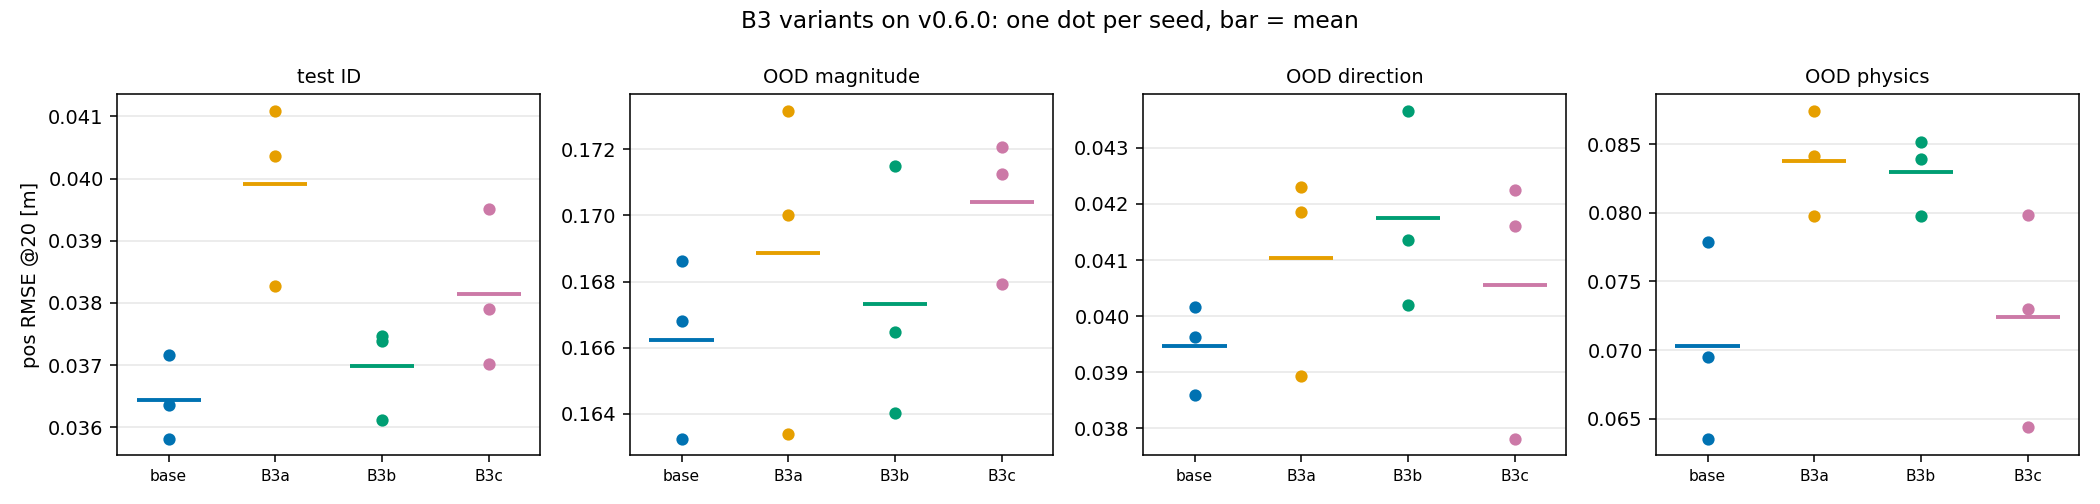
\includegraphics[width=\columnwidth]{figures/b3_variants.png}
\caption{B3 variants per seed: no variant separates from base B3 beyond seed noise.}
\end{figure}

The findings are:
\begin{enumerate}
\item The physics prior helps in distribution: B3 is about three times better than B2 and 1.5 times better than B1, and also best on OOD temporal and gust wind.
\item It does not help on OOD wind magnitude, the primary axis: B3 is about at the level of physics alone, B2 is better, and the oracle wrench shows the information exists (0.018~m).
\item A constant-velocity extrapolation beats every physics-based model on OOD magnitude and direction. This reference was missing from the first comparison; it showed that B5b's good OOD numbers came from picking an almost untrained checkpoint.
\item B4 and B5b degrade as they train; a lower learning rate did not help, and the weight-decay test was too weak to be informative.
\item Three B3 variants (no action in the residual, a zero-residual penalty, a shared trunk) are within seed noise of B3.
\item A ridge probe finds no linearly readable wind-force information in the latent (R$^2\le0$), while torque, used as a positive control, gives 0.8.
\item The IMU correction (v0.5 against v0.6) has no effect beyond seed noise.
\end{enumerate}
A check of a 20~Hz controller and model step showed stable tracking on 12 scenarios with and without wind; position-controlled scenarios were identical to 50~Hz and one attitude-mode scenario was worse (one episode per cell).

\subsection{Challenges and how they were handled}
\begin{itemize}
\item \textbf{Checkpoint bug.} The trainer's best-metric was reset at each curriculum stage, so \texttt{best.pt} was not the best epoch for 8 of 16 runs. An audit found it; the code was fixed with a regression test, earlier statements were corrected and the runs repeated.
\item \textbf{IMU artefact.} A lever-arm explanation was tested and refuted; the residual fits $-\omega\times v$ ($R^2=0.83$). It is corrected at generation.
\item \textbf{Reproducibility.} Episodes depended on earlier episodes in the same process ($\approx 6\times10^{-6}$~m) because realised inertia was computed from float32 world poses before reset. After five wrong hypotheses, a bit-level trace of controller inputs and outputs located the cause; it is fixed.
\item \textbf{Silent failures.} A Dryden profile that produced no turbulence was caught by a unit test; a run that aborted without a traceback because the simulator close kills the process now logs and continues, with checkpointed, resumable output.
\item \textbf{Shared host.} Test timeouts from thread oversubscription and generation memory (6--16~GB per worker) are handled by fixed thread counts, and a fixed worker count on resume.
\end{itemize}

\begin{figure}[t]
\centering
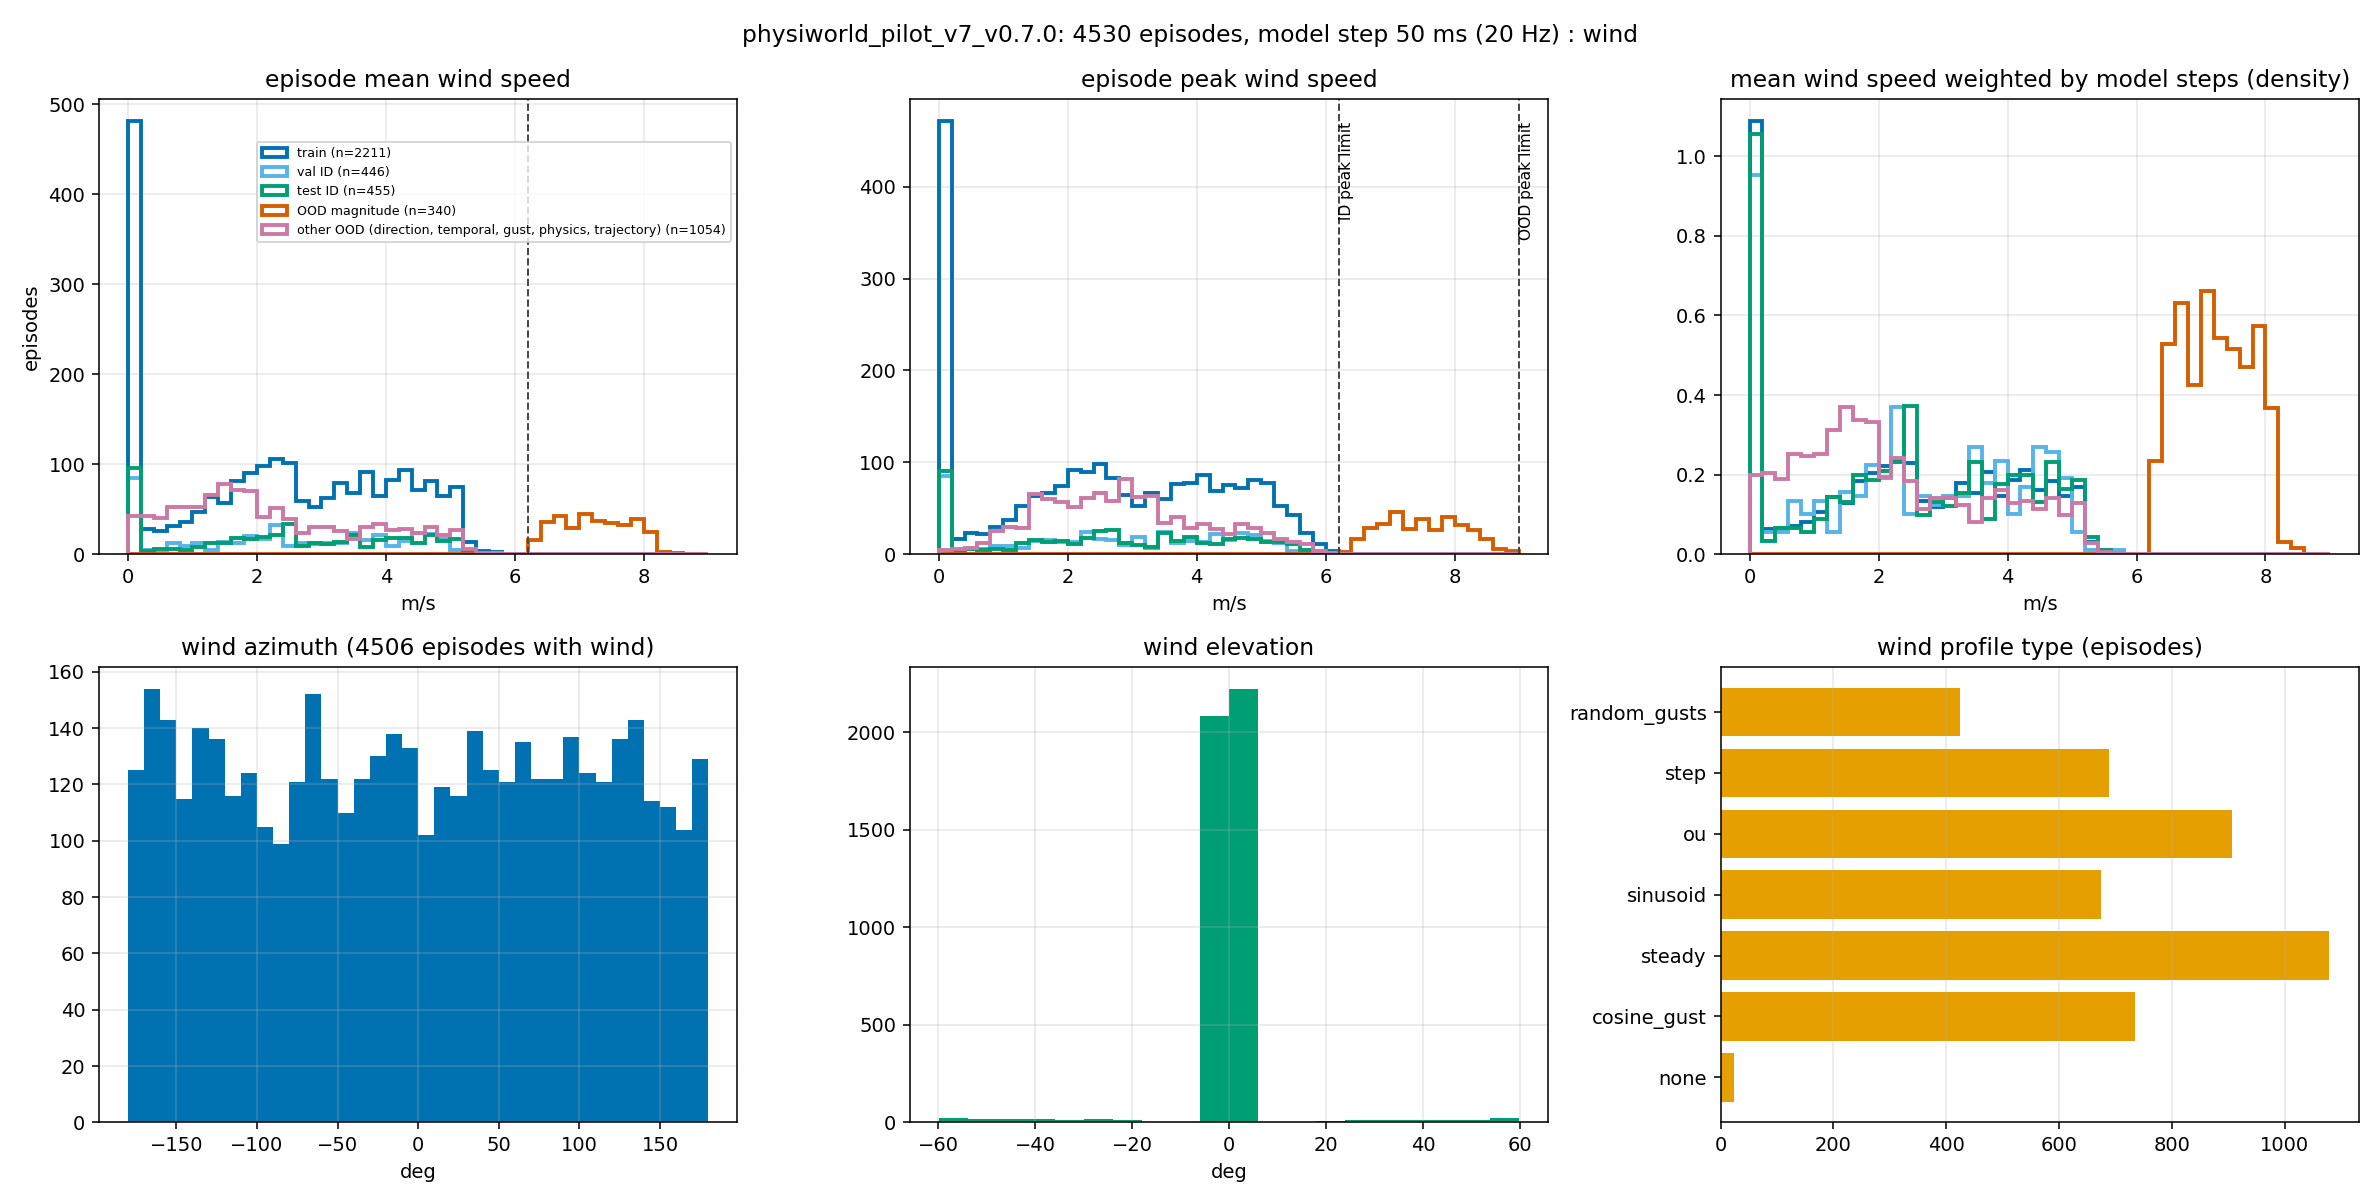
\includegraphics[width=\columnwidth]{figures/v7_wind.png}
\caption{Wind distribution of the pilot-v7 plan (4,530 episodes): stratified, upper-band-weighted in-distribution wind (peak $\le 6.2$~m/s) and OOD magnitude above 6.2~m/s.}
\end{figure}

\subsection{Next-stage dataset}
Training wind in the pilot never exceeded 3.7~m/s while OOD peaks were 4.3--8.2~m/s, so the residual had nothing to extrapolate from. Pilot v7 widens the in-distribution wind to a peak of 6.2~m/s with stratified bands, and OOD to a mean above 6.2~m/s (peak up to 9~m/s). It uses a 50~ms model step and 10~s episodes (20 steps then cover 1~s), 4,530 episodes, about 906k model steps and 473 vehicles, with Mode~B episodes in the test roles and 6--58 vehicle domains per evaluation role. Generation is running on 9 workers with automatic resume; 29.6\% was complete on 26 November.

\section{Future Work}
\begin{enumerate}
\item Finish and validate pilot v7.
\item Retrain B1--B6 on v7 with at least three seeds and a horizon curriculum to 50 steps.
\item Test why the residual does not extrapolate: wind-range augmentation, selection of checkpoints on an OOD validation role, longer history, a stronger weight-decay test (0.1--1), a non-linear probe, and a disturbance-supervision head.
\item Primary experiment (RQ1, RQ2): error growth and reliable imagination horizon of B2 against B3 under OOD wind, with intervals over groups.
\item Ablations (RQ3): physics mismatch, training-data size, latent memory.
\item Optional: uncertainty head (RQ4), ground effect, a second airframe.
\item Thesis writing; update the proposal text where the design changed.
\end{enumerate}

\section{Conclusion}
The infrastructure needed for a trustworthy test of H1 is in place and validated. Early results are mixed: the physics prior helps in distribution but not on strong OOD wind, and a trivial baseline is better there. The remaining work tests the diagnosed causes on a larger dataset and measures long-horizon reliability.

\begin{thebibliography}{9}
\bibitem{gu2024physics} W.~Gu, S.~Primatesta, and A.~Rizzo, ``Physics-informed neural network for quadrotor dynamical modeling,'' \emph{Robotics and Autonomous Systems}, vol.~171, Art.~104569, 2024.
\bibitem{bauersfeld2021neurobem} L.~Bauersfeld, E.~Kaufmann, P.~Foehn, S.~Sun, and D.~Scaramuzza, ``NeuroBEM: Hybrid aerodynamic quadrotor model,'' in \emph{Proc. Robotics: Science and Systems}, 2021.
\bibitem{hafner2023mastering} D.~Hafner, J.~Pasukonis, J.~Ba, and T.~Lillicrap, ``Mastering diverse domains through world models,'' arXiv:2301.04104, 2023.
\end{thebibliography}
\end{document}
